%!TEX root = ../main.tex
\newpage
\section{Decay time resolution and acceptance (3 pages)}
\label{sec:bd2jpsiks:decaytime}

\subsection{Decay time resolution}
\label{sec:bd2jpsiks:decaytime:resolution}

Although the determination of vertices and the measurement of momenta is
pretty accurate at \lhcb (especially thanks to the VELO) a finite resolution
remains which causes a finite decay time resolution. This can dilute the
measured \CP asymmetry but the slow oscillation of \Bd mesons reduces the
impact significantly. Nevertheless, a proper description of the decay time
resolution needs to be found. The most obvious effect of the decay time
resolution are candidates which are reconstructed with negative decay times.
However, these are ideal candidates to determine the decay time resolution. An
unbinned likelihood fit to the decay time distribution of an unbiased
\BdToJPsiKS sample with true \jpsi candidates (selected by a fit of the
invariant $m_{\mumu}$ mass distribution) is performed. The fit model consists
of a component for the prompt peak around \SI{0}{\ps}, \ie the decay time
resolution model, a component to describe events where the wrong PV has been
associated and therefore a large difference between true and reconstructed
decay time occurs, and long lived components which are parametrised with two
exponentials with different pseudo lifetimes and which are themselves
convolved with the decay time resolution model. The decay time resolution
depends on characteristics of the event. The DTF provides predictions for the
per-event decay time resolution $\sigma_t$ which in principle could be used as
width of a Gaussian resolution model. Unfortunately, these predictions are not
perfect and a certain calibration needs to be applied. Additionally, to
account for different sources causing the decay time resolution an effective
model with two Gaussian functions which share a common mean but have different
calibrations is used.

The first step is to find a reasonable calibration model. A linear ($f_1$) and
a quadratic ($f_2$) calibration model are tested:
\begin{equation}
\begin{aligned}
f_1:&\quad \sigma_{\text{true}}(\sigma_t) &=&  &b_i\,\sigma_t &+ c_i \ , \\
f_2:&\quad \sigma_{\text{true}}(\sigma_t) &=&\, \alpha_i\,\sigma_t^2 + &\beta_i\,\sigma_t &+ \gamma_i \ .
\end{aligned}
\label{eq:resolutioncalibfunctions}
\end{equation}
%
The data sample is divided into \num{20} equally filled bins of the decay time
resolution predictions $\sigma_t$. This is done separately for the downstream
and the long track sample as the decay time resolution of long track
candidates is expected to be significantly better. Under the assumption that
$\sigma_t$ is constant inside the bins average widths can be set for the two
Gaussian functions. An unbinned likelihood fit to the decay time distribution,
simultaneous to all bins, sharing all fit parameters except the widths of the
Gaussian resolution functions is performed. The widths are plotted in the
corresponding bins and a \chisq-fit with the two calibration functions is
executed. For the downstream sample the results are depicted in
\cref{fig:CalibrationOffsetResolution_DD}. \todo{replace plots with different line styles}
%
\begin{figure}[!htb]
\centering
  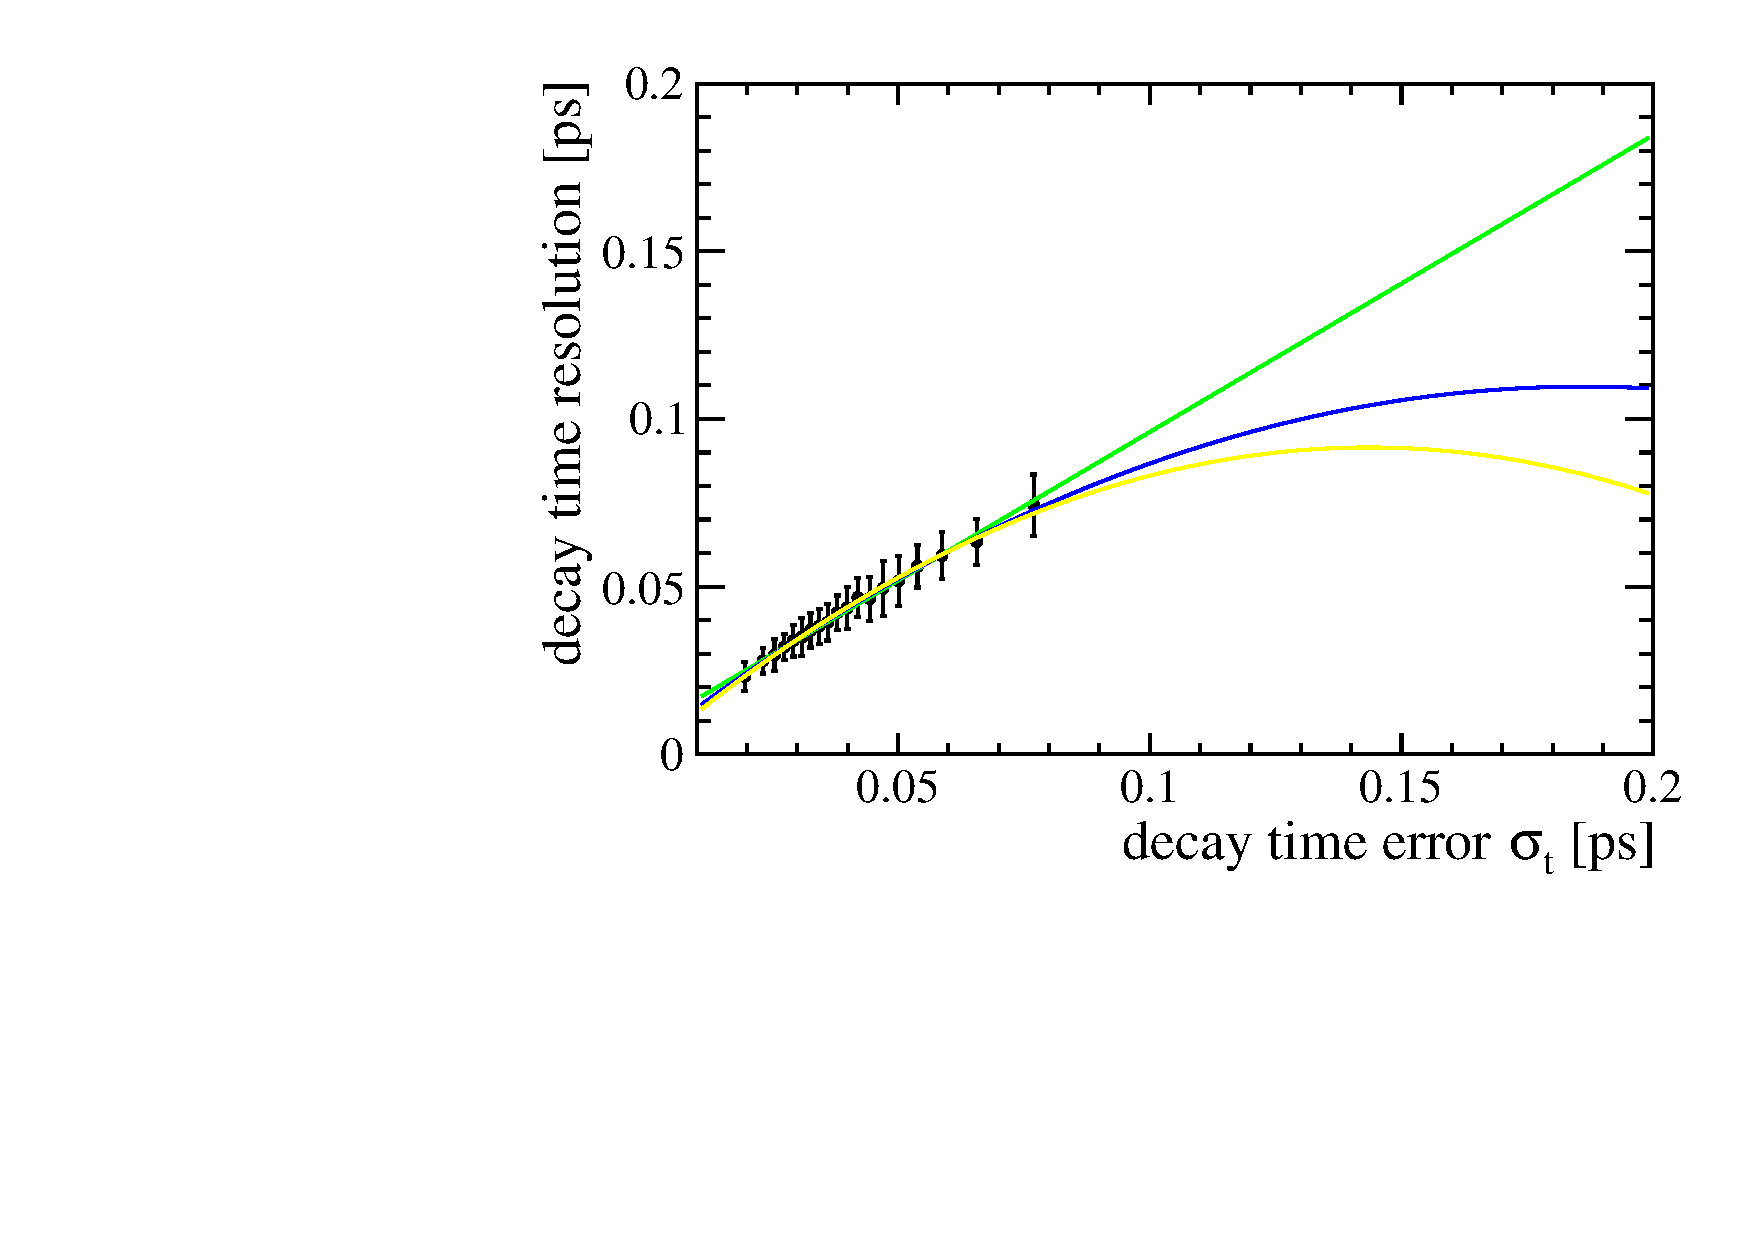
\includegraphics[width=0.45\textwidth]{06-Bd2JpsiKS/figs/ResolutionCalibration_1_DD.pdf}
  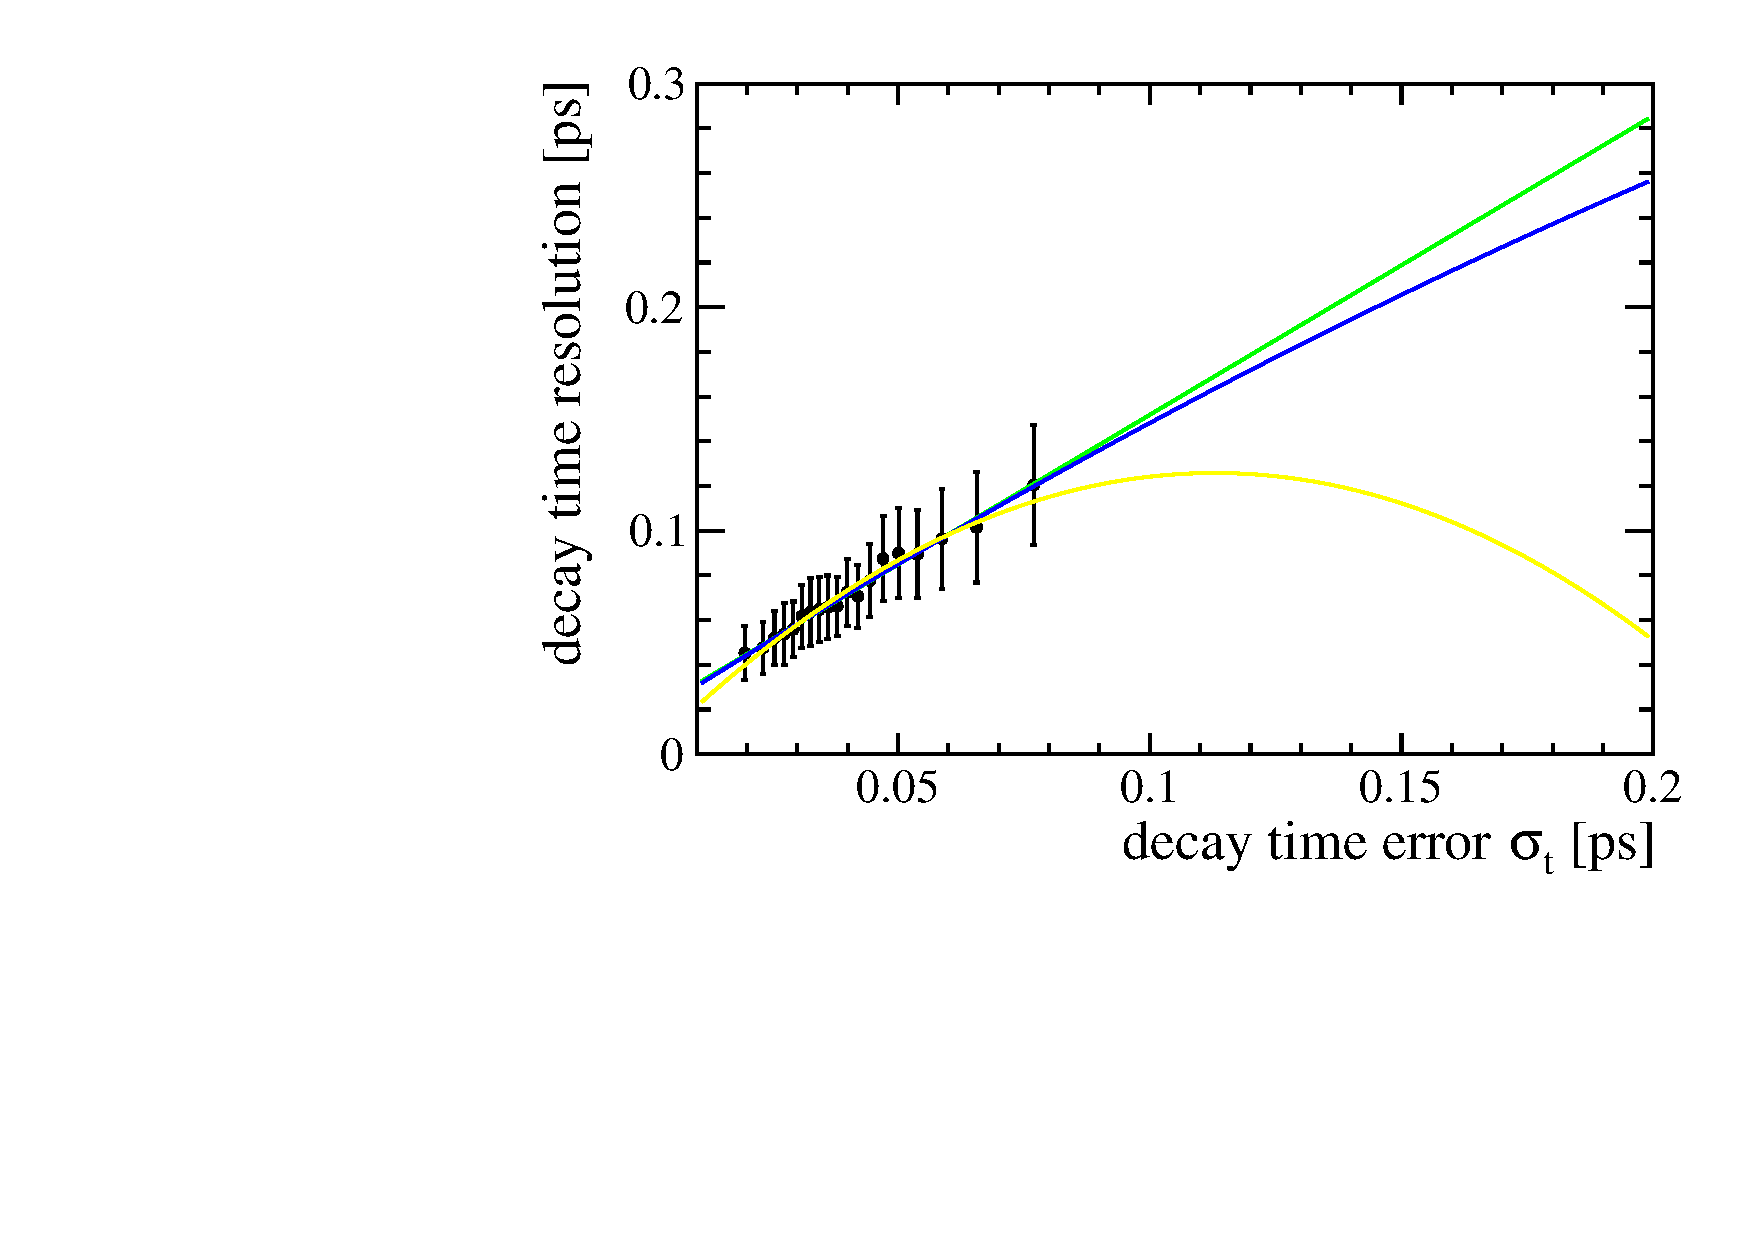
\includegraphics[width=0.45\textwidth]{06-Bd2JpsiKS/figs/ResolutionCalibration_2_DD.pdf}
\caption{Fit of a linear (green) and a quadratic calibration function (blue)
to the narrower (left) and to the wider width (right) of the downstream
sample. Fixing the offset of the quadratic function to zero (yellow) results
in an unphysical shape.}
\label{fig:CalibrationOffsetResolution_DD}
\end{figure}
%
Both functions fit equally well so the simpler linear model with less degrees
of freedom is preferred. The liner model is also chosen for the long track
sample.

With the calibration functions at hand a likelihood fit unbinned in decay
times and decay time resolution predictions is performed and the nominal
values of the calibration parameters are determined. The dilution factor
induced by the decay time resolution is calculated to be \num{0.986} for
downstream and \num{0.989} for long track candidates.

\subsection{Decay time acceptance}
\label{sec:bd2jpsiks:decaytime:acceptance}

The trigger line requirements applied in the selection of the \BdToJPsiKS
candidates partially bias the decay time distribution. The sample is divided
into an \emph{almost unbiased} subset and an \emph{exclusively biased} subset.